\subsection{Beta Negative}
\paragraph{Purpose}
It describes the probability of failures needed to get $r$ successes in a sequence of independent
Bernoulli trials. The probability $p$ remains constant within a given a Bernoulli experiment however
varies across different experiments following a beta distribution.
\paragraph{Theory}
\subparagraph{Parameters}
\begin{itemize}
    \item $\alpha\in\mathbb{R}_{+}$ parameter of Beta distribution
    \item $\beta\in\mathbb{R}_{+}$ parameter of Beta distribution
\end{itemize}
\subparagraph{Probability mass function}
Consider $f_{X|p}(k|r, q)$ the negative binomial density and $f_{p}(q|\alpha,\beta)$ the beta density
we obtain the probability mass function $f(k|\alpha, \beta, r)$ by marginalisation
\begin{align*}
    f(k|\alpha,\beta,r) &= \Su{0}{1}f_{X|p}(k|r,q)\times f_{p}(q|\alpha, \beta)dq\\
                        &= \Su{0}{1}{k+r-1\choose k}(1-q)^{k}q^{r}\times \dfrac{q^{\alpha -1}(1-q)^{\beta -1}}{B(\alpha, \beta)}dq\\
                        &= \dfrac{1}{B(\alpha, \beta)}{k+r-1\choose k}\Su{0}{1}q^{\alpha + r-1}(1-q)^{\beta +k-1}dq\\
                        &= \dfrac{1}{B(\alpha, \beta)}{k+r-1\choose k}\dfrac{\Gamma(\alpha + r)\Gamma(\beta + r)}{\Gamma(\alpha + \beta + k + r)}\\
                        &= \dfrac{1}{B(\alpha, \beta)}{k+r-1\choose k}B(\alpha + r, \beta + k)
\end{align*}
More generally $f(x) = \dfrac{\Gamma(r+k)}{k!\Gamma(r)}\times\dfrac{B(\alpha + r, \beta + k)}{B(\alpha,\beta)}$

\subsection{Boltzmann}
\paragraph{Purpose}
This distribution known as well as Gibbs distribution describes the probability that a system will be
in certain state as a function of that state's energy and the temperature of the system.
\paragraph{Theory}
\subparagraph{Parameters}
\begin{itemize}
    \item $\epsilon_{i}$ the energy of the state $i$
    \item $k$ the Boltzmann constant 
    \item $T$ the temperature
\end{itemize}
\begin{figure}[H]
    \begin{center}
        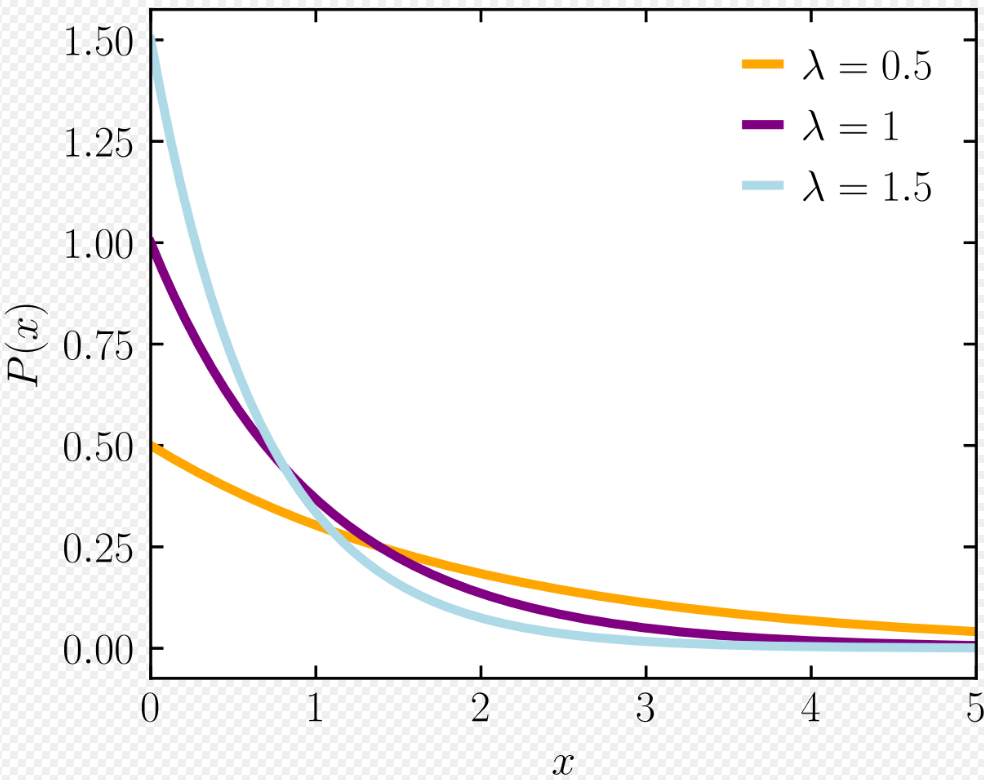
\includegraphics[width=.5\textwidth]{./chapters/2_statistics/02_common_probability_distributions/images/06_boltzman_pmf.png}
    \end{center}
    \caption{Boltzmann probability function, note that $lambda = kT$}
    \label{fig:06_boltzman_pmf}
\end{figure}

\subparagraph{Probability mass function}
Assume $p_{i}$ the probability of the system being in state $i$, 
$p_{i}\propto e^{-\frac{\epsilon_{i}}{kT}}$.\\ 
More precisely we have $f(i) = \prob{X=i} = \dfrac{e^{-\frac{\epsilon_{i}}{kT}}}{\su{j=1}{M}e^{-\frac{\epsilon_{j}}{kT}}}$


\subsection{Borel}
\subsection{Discrete phase-type}
\subsection{Extended negative binomial}
\subsection{Geometric}
\subsection{Mixed Poisson}
\subsection{Negative binomial}
\subsection{compound Poisson}
\subsection{Poisson}
\subsection{Skellam}
\subsection{Zeta}
